\documentclass[11pt]{article}
\usepackage[utf8]{inputenc}
\usepackage{polski}
\usepackage{graphics}
\usepackage[demo]{graphicx}
\graphicspath{{images/}}
\usepackage[section]{placeins}
\usepackage{fullpage}

\title{Metody Numeryczne Projekt 2}
\author{Martyna Kuśmierz\\Grupa nr 2}
\date{11.01.2023r}

\begin{document}

\maketitle

\section{Polecenie}

\begin{figure}[h]
    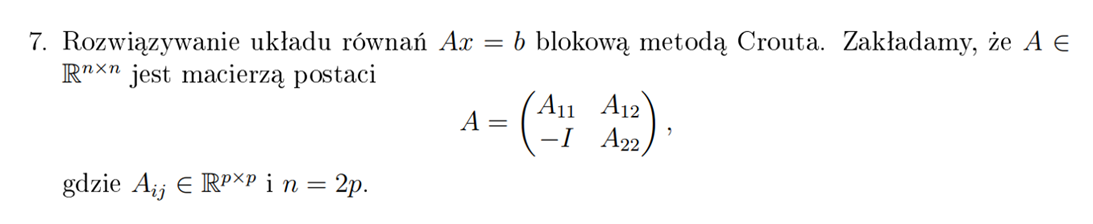
\includegraphics[scale=0.7]{Polecenie.png}
    \centering
    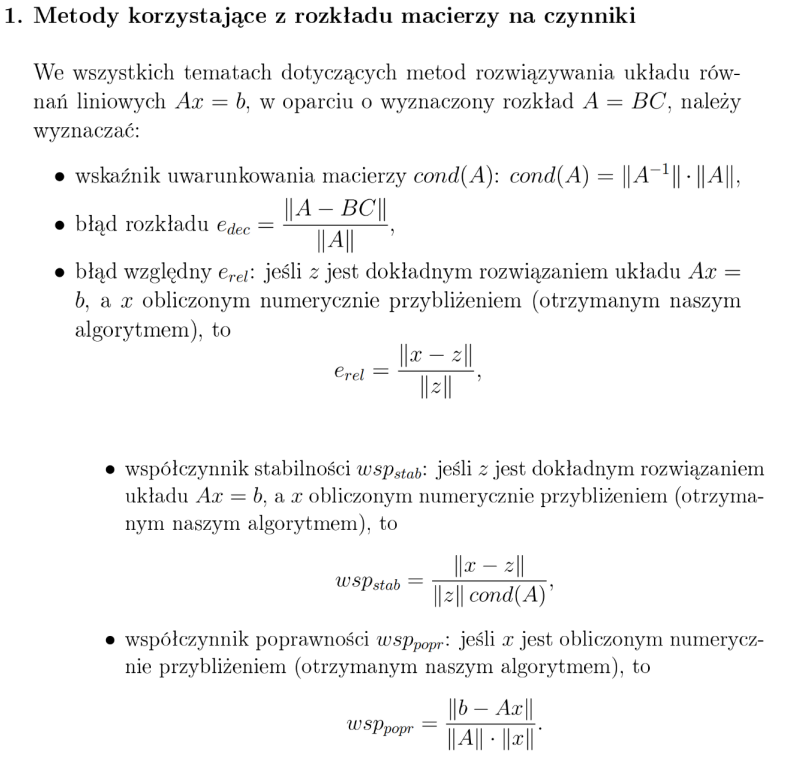
\includegraphics[scale=0.7]{Polecenie2.png}
\end{figure}

\section{Opis metody}
Blokowa metoda Crouta polega na rozkładzie LU macierzy, gdzie macierz U posiada macierze jednostkowe na przekątnej. Następnie wykorzystujemy ten rozkład do rozwiązania układów liniowych.
\begin{figure}[h]
    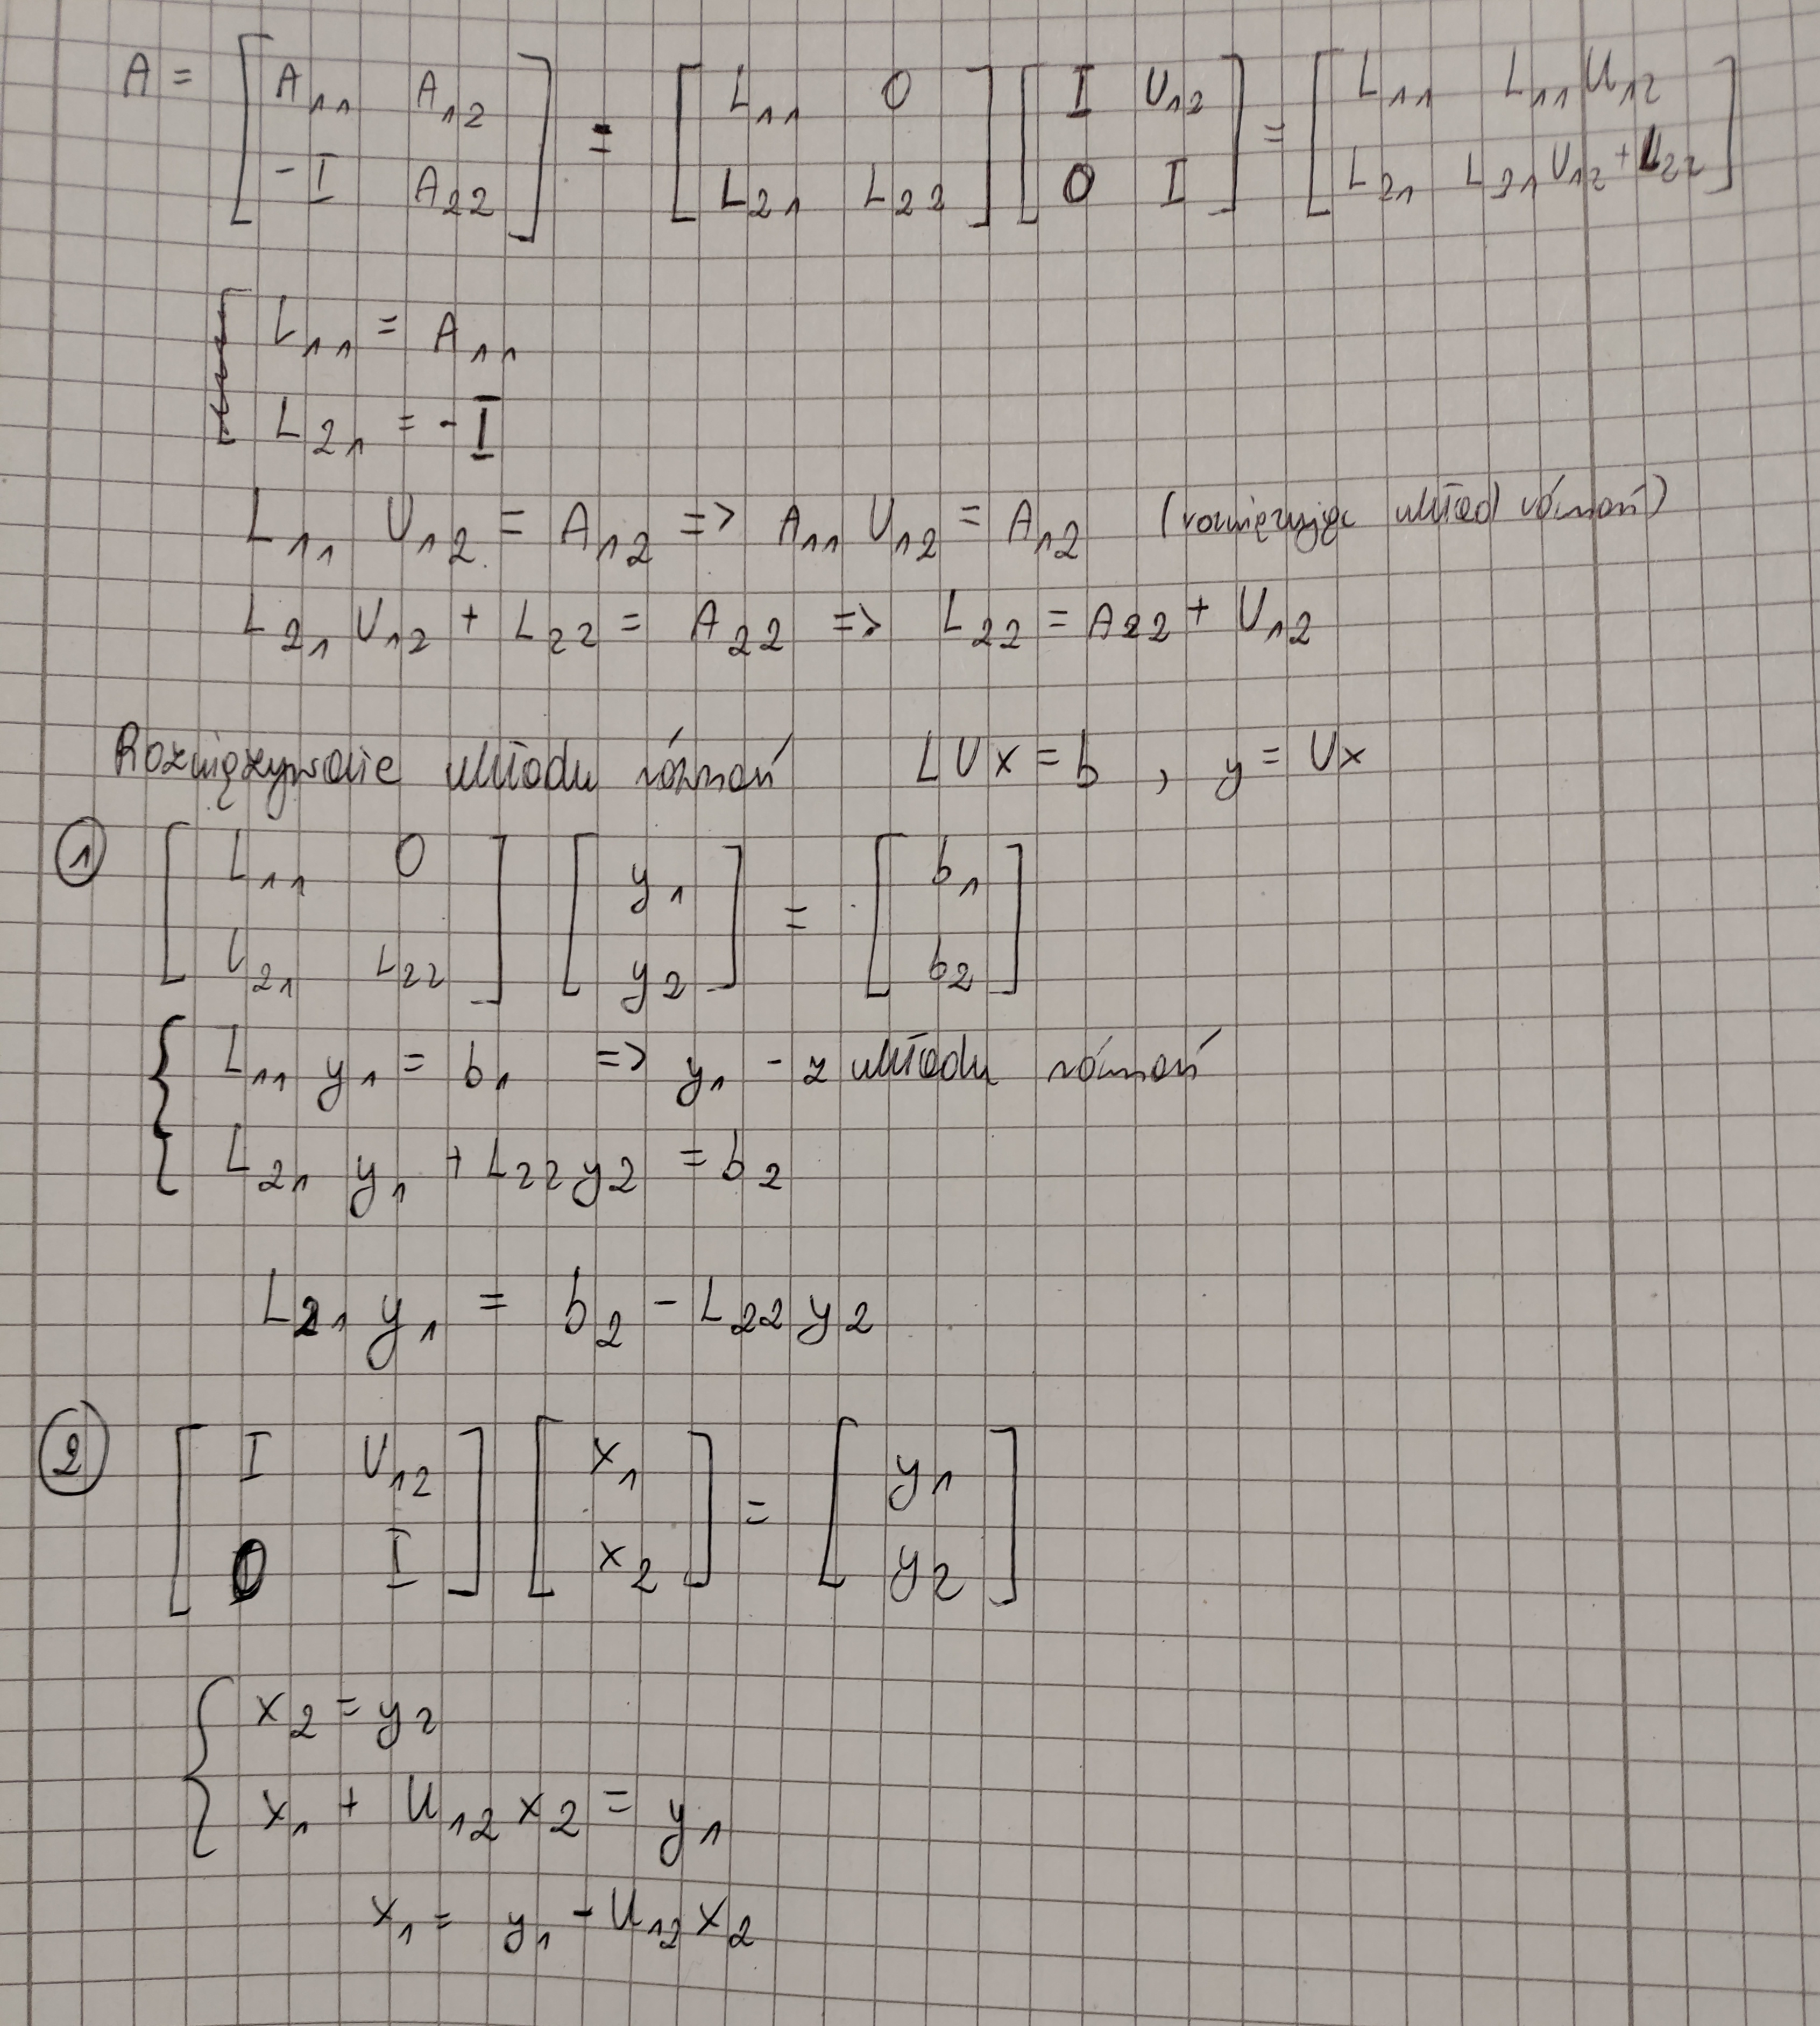
\includegraphics[scale=0.12]{metoda.jpg}
    \centering
\end{figure}

\break
\section{Opis programu}

Program składa się ze skryptu oraz 2 funkcji.
\begin{itemize}
\item function [x] = Crout(A, b)
\newline
Funkcja wykonuje rozkład macierzy A, LU w postaci Crouta oraz rozwiązuje układ liniowy LUx = b.\\
Parametry wejścia:
\begin{enumerate}
  \item A - macierz $R^{nxn}$
  \item b - wektor układu $R^n$
\end{enumerate}
Parametry wyjścia:
\begin{enumerate}
  \item x - wektor rozwiązania $R^n$
\end{enumerate}
\item function [x] = BlockCrout(A,b)\\
Funkcja rozwiązuje układ liniowy metodą blokową Crouta. Wykorzystuje funkcję Crout(A,b) do rozwiązywania układów równań. Dodatkowo wypisuje takie informacje jak:
\begin{enumerate}
    \item wskaźnik uwarunkowania macierzy
    \item błąd rozkładu
    \item błąd względny
    \item współczynnik stabilności
    \item współczynnik poprawności
\end{enumerate}
Parametry wejścia:
\begin{enumerate}
  \item A - macierz $R^{nxn}$
  \item b - wektor układu $R^n$
\end{enumerate}
Parametry wyjścia:
\begin{enumerate}
  \item  x - wektor rozwiązania $R^n$
\end{enumerate}
\item Skrypt\\
W skrypcie znajdują się przykładowe macierze oraz wektory i wywołanie dla nich funkcji BlockCrout(A,b). Dodatkowo wynik jest porównywany z wbudowaną funkcją w Matlabie.
\end{itemize}

\break
\section{Przykłady}
\begin{enumerate}

    \item W przypadku poniższej macierzy A wyniki różnią się w miejscu zaokrąglenia. X to wynik obliczony za pomocą algorytmu, a ans to wynik obliczony za pomocą wbudowanej funkcji w Matlabie.
    
    \begin{figure}[h]
        \centering
        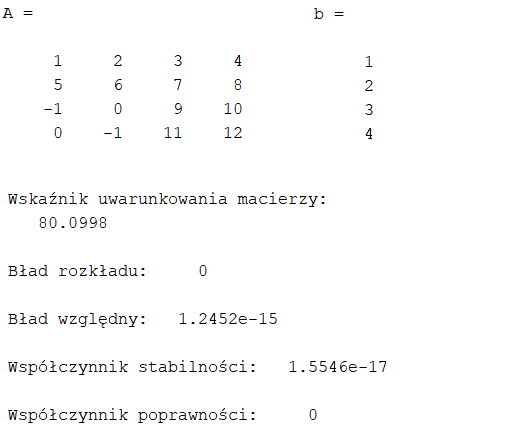
\includegraphics[scale=0.8]{A1}
        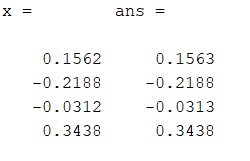
\includegraphics[scale=0.9]{A2}
    \end{figure}


    \item Podmacierze macierzy B są macierzami hilberta. Wektor b jest ten sam. Błędy rozkładu i względne są bardzo niewielkie.

    \begin{figure}[h]
     \centering
     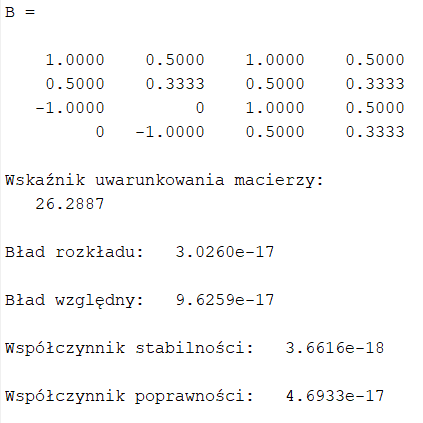
\includegraphics[scale=0.8]{B1}
     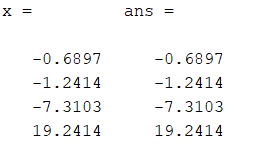
\includegraphics[scale=0.9]{B2}
    \end{figure}

    \break
  

    \item Macierz C podobnie jak macierz B składa się z macierzy hilberta. Jej wskaźnik uwarunkowania jest większy niż w przypadku poprzedniej macierzy. Błędy są jednak porównywalne.
    \begin{figure}[h]
        \centering
        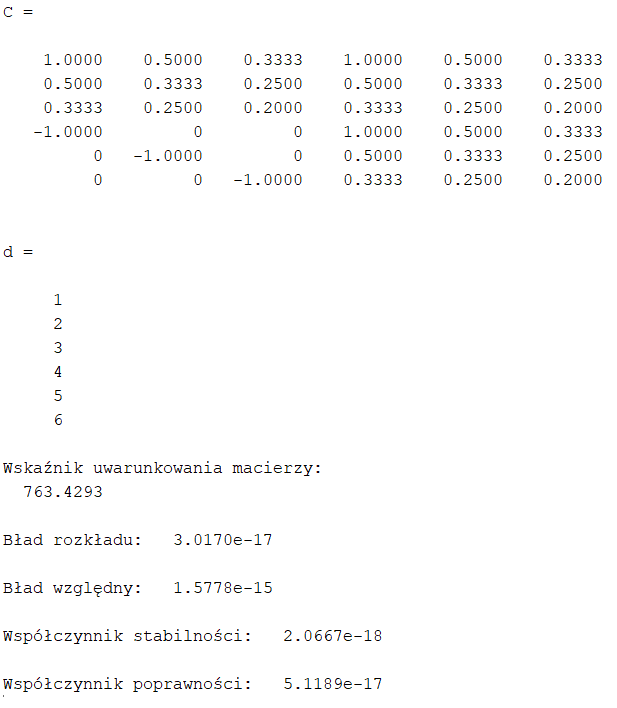
\includegraphics[scale=0.8]{C1}
        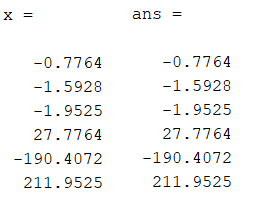
\includegraphics[scale=0.9]{C2}
    \end{figure}
    
    \break

    \item Podmacierze macierzy D składają się z macierzy Pascala. Wskąźnik uwarunkowania jest niewielki, a wszystkie współczynniki wynoszą 0.
    \begin{figure}[h]
        \centering
        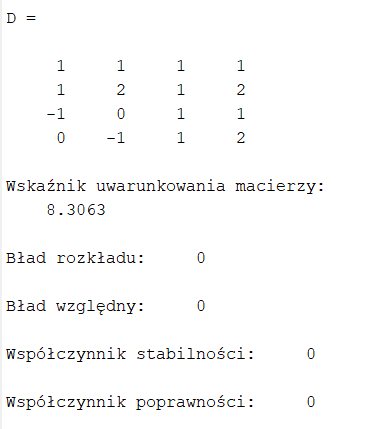
\includegraphics[scale=0.8]{D1}
        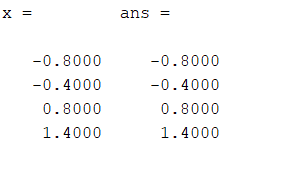
\includegraphics[scale=0.9]{D2}
    \end{figure}


    \item Wyznacznik macierzy E wynosi 0. Program jednak nie obsługuje macierzy osobliwych.
    \begin{figure}[h]
        \centering
        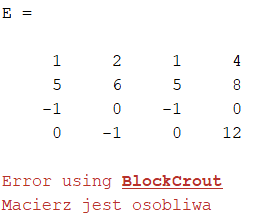
\includegraphics[scale=0.8]{E1}
    \end{figure}

    \break

    \item Macierz F jest macierzą o bardzo wysokim wskaźniku uwarunkowania. Niewielka zmiana w wektorze c1 powoduje znaczącą zmianę wyniku.
    \begin{figure}[h]
        \centering
        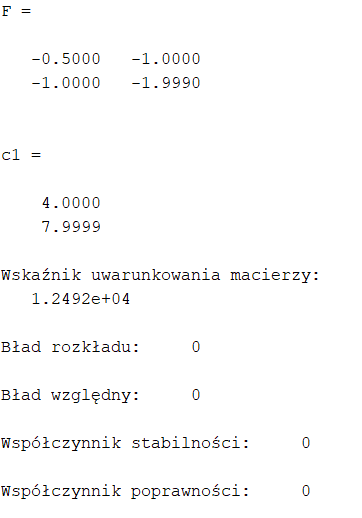
\includegraphics[scale=0.8]{F1}
        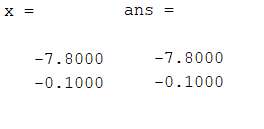
\includegraphics[scale=0.9]{F2}\\
        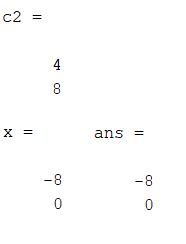
\includegraphics[scale=0.8]{F3}
    \end{figure}


\end{enumerate}

\section{Analiza wyników}
Przy użyciu algorytmu otrzymujemy identyczne wyniki jak w przypadku wbudowanej funkcji w Matlabie do rozwiązania układu równań liniowych. Niemożliwe jest rozwiązanie układu dla macierzy osobliwych. Błędy rozkładów poszczególnych macierzy są bardzo niewielkie lub zerowe. Uzyskujemy prawidłowe wyniki również dla macierzy o wysokim wskaźniku uwarunkowania.

\end{document}


